% GENERATED by reporting/make_priors_report.py -- do not edit by hand.
% Source: metrics/outputs/{toy-temporal,gemma-2-2b*}/ -- frozen run results, not prose.
% Every caption is TODO on purpose: a caption is a claim about what to take away,
% and this project requires those to be written by a person.
% Regenerate:  python3 -m reporting.make_priors_report
% Requires:    \input{thresholds_macros.tex} in the preamble (defines \MinJoint etc.),
%              and packages booktabs, graphicx, amsmath.


% ------------------------------------------------------------------------
% Toy model
% ------------------------------------------------------------------------

% [toy-boundary]
\begin{figure}[tbp]
  \centering
  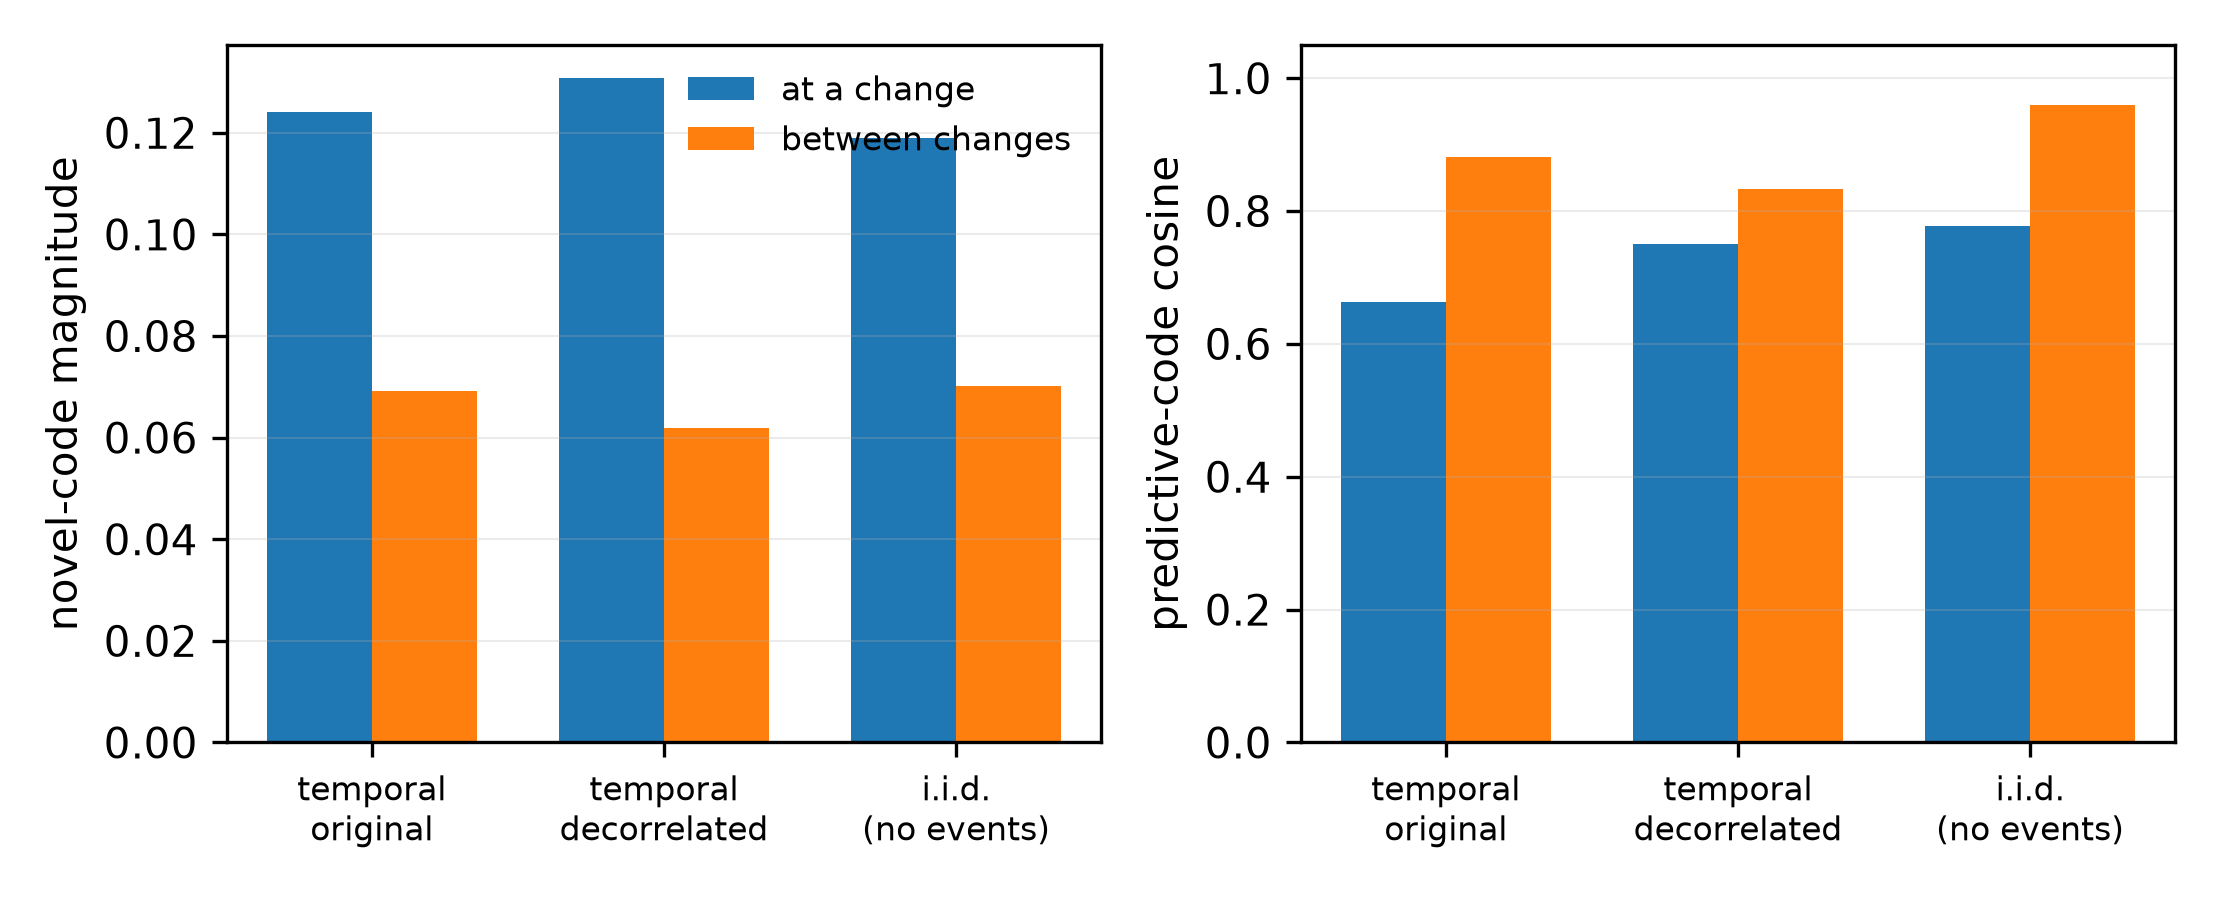
\includegraphics[width=\linewidth]{figuers/pit_boundary}
  \caption{TODO(caption, human-written). The same measurements, drawn. The control row has no planted changes in it at all, so it shows what these measures do when there is nothing to find.}
  \label{fig:pit-boundary}
\end{figure}
